\documentclass[a4paper, 12pt]{article}
\usepackage{arxiv}
\usepackage[T2A]{fontenc}
\usepackage[utf8]{inputenc}
\usepackage[english, russian]{babel}
\usepackage{url}
\usepackage{booktabs}
\usepackage{amsfonts}
\usepackage{nicefrac}
\usepackage{microtype}
\usepackage{lipsum}
\usepackage{graphicx}
\usepackage{natbib}
\usepackage{doi}
\usepackage{amsthm}
\usepackage{svg}
\usepackage[utf8]{inputenc}
\usepackage{amsmath}
\usepackage{mathtools}
\usepackage{extsizes} % Возможность сделать 14-й шрифт
\newtheorem{theorem}{Теорема}
% \renewcommand{\shorttitle}{\textit{arXiv} Template}
\renewcommand{\headeright}{}
\renewcommand{\undertitle}{}
\renewcommand{\abstractname}{Аннотация}
\newcommand{\keywordsname}{Ключевые слова:}

\begin{document}
\title{Выбор интерпретируемых рекуррентных моделей глубокого обучения}
\author{\normalsize\bf{Гапонов Максим,~Бахтеев Олег,~Яковлев Константин,~Стрижов Вадим} \\
	Московский физико-технический институт \\
	\texttt{\{gaponov.me,~bakhteev,~strijov\}@phystech.edu}
}
\date{}
\maketitle
\begin{abstract}
Рассматривается задача интерпретации рекуррентных нейронных сетей. Под интерпретируемостью модели понимается возможность получить линейную зависимость выходных данных от входных. Предлагается обобщить метод OpenBox, предназначенный для интерпретации нейронных сетей с кусочно-линейными функциями активации. В данном методе нейронная сеть представляется в виде ансамбля интерпретируемых линейных классификаторов, каждый из которых определён на выпуклом многограннике, поэтому интерпретации близких объектов согласованны. Для анализа качества предложенного метода проводится эксперимент на выборке IMDB Review dataset.
\end{abstract}
\renewcommand{\abstractname}{Abstract}
\begin{abstract}
The problem of interpretation of recurrent neural networks is considered. The interpretability of the model is understood as the ability to obtain a linear dependence of the output data on the input data. It is proposed to generalize the OpenBox method designed for the interpretation of neural networks with piecewise linear activation functions. In this method, the neural network is represented as an ensemble of interpreted linear classifiers, each of which is defined on a convex polyhedron. Therefore, the interpretations of close objects are consistent. To test the operability of the proposed method, an experiment is conducted on a sample of the IMDB Review dataset.
\end{abstract}

\keywords{Интерпретация моделей \and Рекуррентные нейронные сети \and Кусочно-линейные модели}

\section{Введение}
В работе рассматривается метод интерпретации рекуррентных моделей глубокого обучения. Такие модели используются для обработки последовательностей данных \cite{lipton2015critical}. Однако из-за большого числа слоёв в нейронной сети она работает по принципу "чёрного ящика". То есть нет явной зависимости выходных данных от входных. Работа посвящена построению и выбору интерпретируемых моделей для рекуррентных нейронных сетей с кусочно-линейными функциями активации.

Рекуррентная нейронная сеть представляет последовательность слоёв нейронов: входного слоя, скрытых слоёв и выходного слоя \cite{sherstinsky2020fundrnn}. Отличительной особенностью от нейронных сетей являются циклические связи между нейронами. Такие связи позволяют запоминать состояния для обработки последовательностей данных.

Интерпретация должна быть \textbf{точной} и \textbf{согласованной} \cite{chu2019exact}. Интерпретация называется точной, если предсказания интерпретируемой модели похожи на предсказания исходной. Интерпретация называется согласованной, если интерпретации близких объектов похожи, то есть значимости признаков близки.

Анализ зависимости предсказания модели от входных данных в рекуррентных нейронных сетях --- открытая проблема. Методы, рассмотренные в работах \cite{dosovitskiy2016inverting, zhou2018interpreting, NIPS2014_ea8fcd92, bastani2019interpreting, zhou2015learning, simonyan2014deep} являются либо неточными, то есть построенные интерпретируемые модели не отвечают поведению исходной модели, либо несогласованными, то есть значимости признаков для близких объектов значительно отличаются.

В работах \cite{dosovitskiy2016inverting, zhou2018interpreting} рассмотрены методы, основанные на интерпретации признаков, выученных скрытыми слоями. Такой подход отражает поведение скрытых слоёв, но не показывает поведение сети в целом. В работах \cite{NIPS2014_ea8fcd92, bastani2019interpreting} предлагаются методы подражания модели. В этом подходе строится модель с похожим на исходную поведением. Построенная модель имеет более простую структуру, поэтому проще интерпретируется. Однако из-за недостаточно сложной структуры построенная модель плохо приближает исходную. Наконец, в работах \cite{zhou2015learning, simonyan2014deep} рассмотрены методы локальной интерпретации, в которых происходит анализ поведения модели в окрестности исходного объекта. В таком подходе получается точная интерпретация одного объекта, однако интерпретации близких объектов могут существенно отличаться. Таким образом, данный подход не предоставляет согласованные интерпретации.

Предложенный в данной работе подход является обобщением метода OpenBox, предназначенного для интерпретации нейронных сетей с кусочно-линейными  функциями активации \cite{chu2019exact}. Нейронная сеть представляется в виде ансамбля линейных классификаторов. Каждый из них классифицирует объекты внутри выпуклого многогранника в пространстве признаков, поэтому интерпретации получаются согласованными.

На выборке IMDB Movie Review Dataset \cite{maas-EtAl:2011:ACL-HLT2011} проведён вычислительный эксперимент для анализа качества метода, а также для проверки интерпретаций на точность и согласованность. 

\section{Задача выбора интерпретируемых моделей}
Рассмотрим рекуррентную нейронную сеть $\mathbf{f}(\mathbf{x})$ с кусочно-линейными функциями активации. Входные данные обозначим через $\mathbf{x} \in \mathbf{X}$, где $\mathbf{X} \subset \mathbb{R}^d$ --- пространство признаков. Выходные данные обозначим через $\mathbf{y} \in \mathbf{Y}$, где $\mathbf{Y} \subset \mathbb{R}^k$ --- пространство предсказаний.

Модель является функцией $\mathbf{f}: \mathbf{X} \to \mathbf{Y}$. Из-за большого числа параметров невозможно получить явную зависимость значения функции $\mathbf{f}$ от аргумента $\mathbf{x}$.

Требуется построить модель, соответствующую функции $\mathbf{g}$, которая обладает следующими свойствами.

Во-первых модель должна быть интерпретируемой. То есть можно построить линейную зависимость выходных данных от входных.

Также модель должна быть точной, то есть минимизировать \eqref{ft:exactness}

\begin{equation}\label{ft:exactness}
\int\limits_{\mathbf{X}}^{}{\left(\mathbf{f}(\mathbf{x}) - \mathbf{g}(\mathbf{x})\right)^2dx} \to \min_{\mathbf{g}}
\end{equation}

Модель должна быть согласованной, то есть должно выполняться \eqref{ft:consistensy}
\begin{equation}\label{ft:consistensy}
\exists \varepsilon > 0\: \forall \mathbf{x}_1, \mathbf{x}_2 \in \mathbf{X}\: ||\mathbf{x}_1-\mathbf{x}_2||<\varepsilon \implies \frac{\partial{\mathbf{g}}}{\partial{\mathbf{x}}}(\mathbf{x}_1)=\frac{\partial{\mathbf{g}}}{\partial{\mathbf{x}}}(\mathbf{x}_2)
\end{equation}

\section{Интерпретация рекуррентных нейронных сетей}

\subsection{Метод OpenBox}

Рассмотрим рекуррентную нейронную сеть $\mathbf{f}(\mathbf{x})$. Она представима в виде нейронной сети, если заменить рекуррентные слои на последовательность обыкновенных слоёв нейронов. А именно, пусть дан слой рекуррентной нейронной сети состоящий из $n$ нейронов с кусочно-линейной функцией активации $f_i$. Обозначим число рекуррентных запусков данного слоя через $k$. Заменим в архитектуре нейронной сети данный слой на $k$ слоёв, состоящих из $n$ нейронов, с функциями активации $f_i$. Таким образом, нейронная сеть представляется в виде обыкновенной сети.

Для слоя с номером $i$

$\mathbf{a}_i~-$ вход слоя

$\mathbf{h}_i~-$ скрытое состояние

$f_i~-$ функция активации

$\mathbf{W}_i~-$ матрица линейного преобразования

$\mathbf{b}_i~-$ вектор сдвига

Рекуррентная нейронная сеть задаётся соотношением \eqref{fm:rnn}

\begin{equation}\label{fm:rnn}
[\mathbf{a}_{i+1}, \mathbf{h}_{i+1}]=f_i\left(\mathbf{W}_i [\mathbf{a}_{i},\mathbf{h}_i] + \mathbf{b}_i\right)
\end{equation}

Рассматриваются кусочно-линейные функции активации, то есть

\[f_i(x)=\left\{
\begin{array}{ll}
      r_1 x+t_1 & \text{if } x\in I_1 \\
      r_2 x+t_2 & \text{if } x\in I_2 \\
      \dots&\dots\\
      r_u x+t_u & \text{if } x\in I_u \\
\end{array} 
\right. \]

Где $I_1,\dots,I_u~-$ разбиение $\mathbb{R}$.

Для фиксированных входных данных $\mathbf{x}$ каждая кусочно-линейная функция $f_i$ является линейной в некоторой окрестности своего аргумента.

Также условие принадлежности аргумента $x$ интервалу $I_j~-$ это неравенство вида $p \leq x \leq q$.

\begin{theorem}
Пусть дана нейронная сеть $\mathbf{f}(\mathbf{x})$ с кусочно-линейными функциями активации $f_i$. Тогда она представима в виде набора линейных функций $F_1,\dots,F_n$, каждая из которых определена на выпуклом многограннике $P_1,\dots,P_n \subset \mathbf{X}$.
\end{theorem}
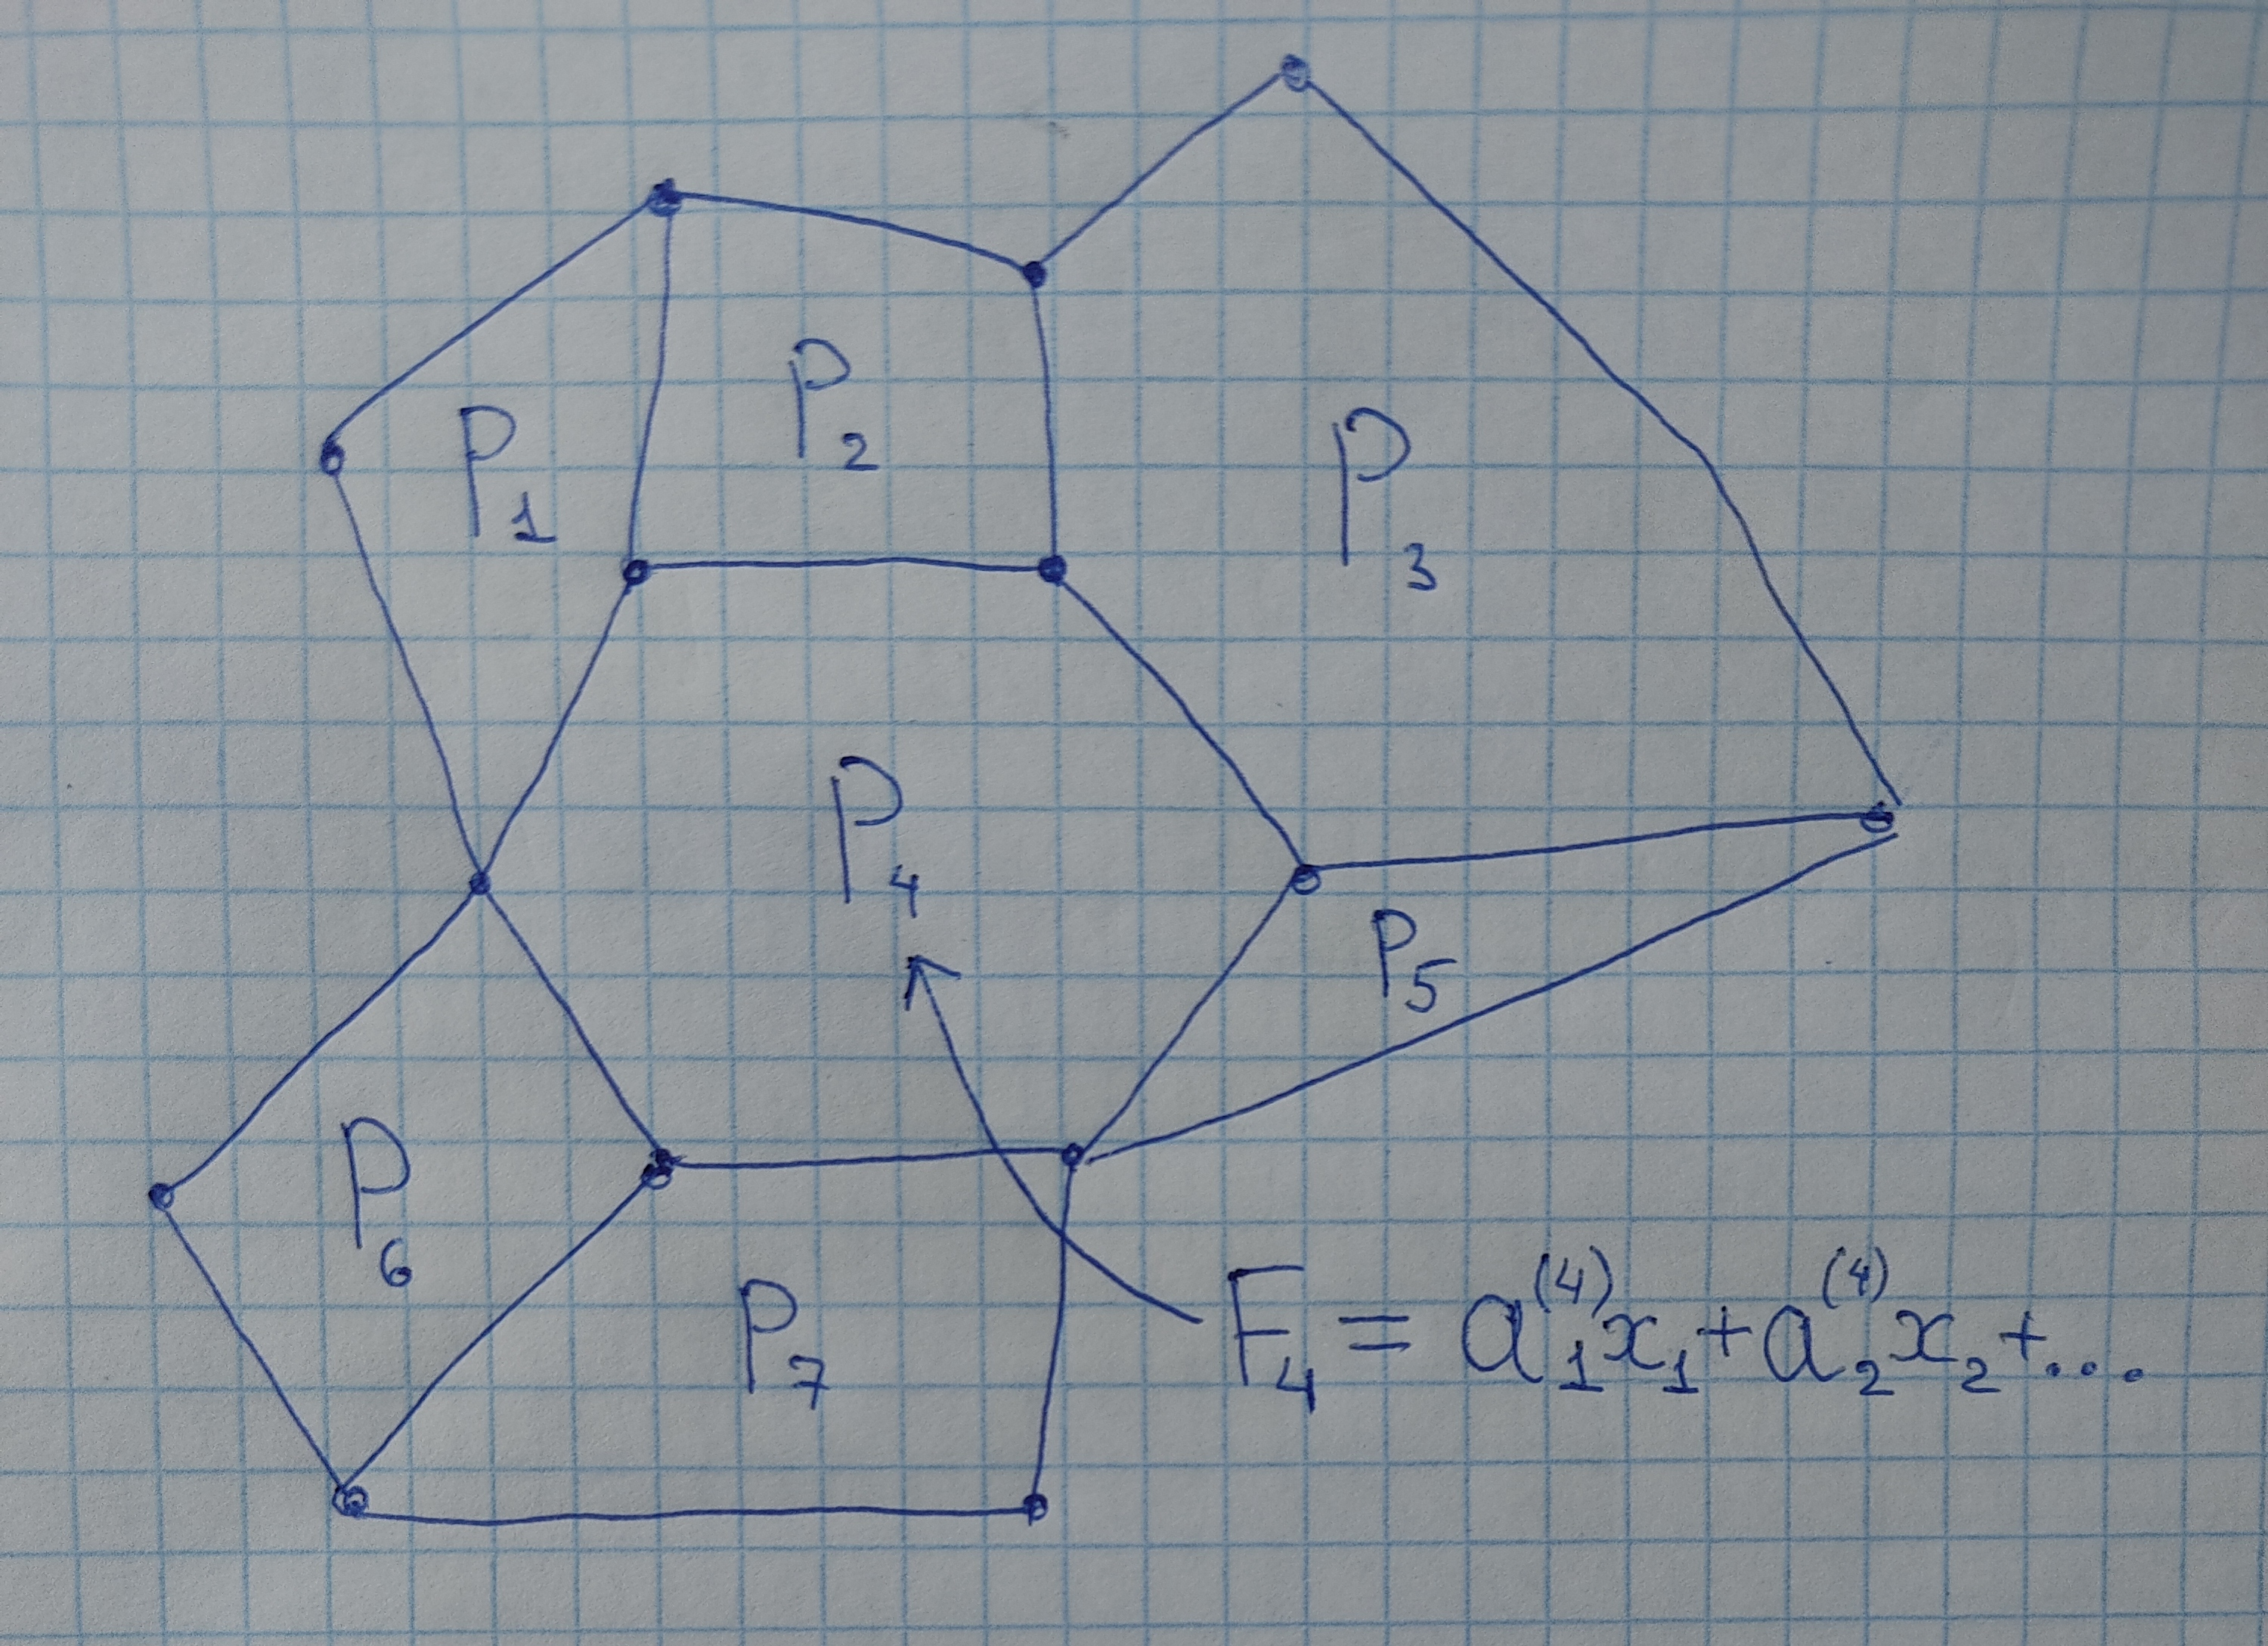
\includegraphics[width=0.95\textwidth]{../figures/polys.jpg}
\begin{proof}
Рассмотрим произвольный $\mathbf{x}_0\in\mathbf{X}$. Кусочно-линейные функции активации $f_i$ являются линейными в некоторой окрестности своего аргумента. Причём условие принадлежности аргумента функции $f_i$ к интервалу $I_j~-$ это пересечение двух линейных неравенств, каждое из которых задаёт полупространство в пространстве $\mathbf{X}$. Пересечением такого семейства полупространств является выпуклый многогранник. Помимо этого, композиция линейных функций является линейной функцией.

Таким образом, найден выпуклый многогранник $P_h$ (пересечение семейства полупространств) и линейная функция $F_h$ (композиция линейных функций) такая, что выполнено следующее

$$\forall \mathbf{x}\in P_h\; \mathbf{f}(\mathbf{x})=F_h(\mathbf{x})$$

В силу произвольности выбора $\mathbf{x}_0$ получаем, что всё пространство $\mathbf{X}$ разбивается на выпуклые многогранники $P_h$, на которых заданы линейные функции $F_h$.

Нейронная сеть $\mathbf{f}$ имеет конечное число нейронов, значит, имеется конечное число неравенств, задающих полупространтва в пространстве $\mathbf{X}$. А конечное число неравенств задает лишь конечное число выпуклых многогранников. 
\end{proof}

Для решения задачи интерпретации рекуррентных нейронных сетей с кусочно-линейными функциями активации предлагается следующим алгоритм.

1. Вычислить коэффициенты линейного классификатора $F_h$, ($h$ такое, что $\mathbf{x}_0\in P_h$) по формуле $\frac{\partial\mathbf{f}}{\partial\mathbf{x}}(\mathbf{x}_0)$

2. Выделить линейные неравенства на $\mathbf{x}_0$, соответствующие выпуклому многограннику $P_h$.

3. Интерпретацией модели на входном объекте $\mathbf{x}_0$ является набор коэффициентов линейного классификатора $F_h$, соответствующие им признаки, а также набор условий задающих $P_h$.

Полученная интерпретируемая модель оказывается математически эквивалентна исходной, то есть выполнено свойство точности \eqref{ft:exactness}.

Также модель обладает свойством согласованности \eqref{ft:consistensy}, так как близкие объекты попадают в один и тот же выпуклый многогранник $P_h$, а значит, классифицируются одним и тем же линейным классификатором $F_h$.

\subsection{Метод LIME}

Рассмотрим метод LIME \cite{ribeiro2016why} для выбора интерпретируемых моделей.

Алгоритм построения интерпретируемой модели $\mathbf{g}(\mathbf{x})$

0. Фиксируются константы $n$ и $K$.

1. Порождаются объекты $\mathbf{x}_1, \mathbf{x}_2, \dots, \mathbf{x_n}$ в окрестности $\mathbf{x}$.

2. Вычисляются предсказания $\mathbf{y}_1, \mathbf{y}_2, \dots, \mathbf{y}_n$ модели $\mathbf{f}$ на объектах $\mathbf{x}_1, \mathbf{x}_2, \dots, \mathbf{x}_n$. То есть $\mathbf{y}_i=\mathbf{f}(\mathbf{x}_i)$.

3. Построение линейной модели $\mathbf{g}(\mathbf{x})$ с $K$ параметрами происходит при помощи метода наименьших квадратов для объектов $\mathbf{x}_1, \mathbf{x}_2, \dots, \mathbf{x}_n$ и соответствующих им меток $\mathbf{y}_1, \mathbf{y}_2, \dots, \mathbf{y}_n$.  

\section{Вычислительный эксперимент}

В рамках эксперимента рассматривается задача классификации отзывов на ресурсе IMDB. Используется выборка IMDB Movie Review Dataset \cite{maas-EtAl:2011:ACL-HLT2011} состоящяя из 50 000 отзывов, а также типов отзывов: положительный, отрицательный. Требуется по тексту отзыва определить вероятность принадлежности отзыва к классу положительных и отрицательных.

Для решения задачи используется рекуррентная нейронная сеть $\mathbf{f}$ \eqref{fm:rnn},
аргументом которой являются последовательности предобученных векторов эмбедингов слов отзыва. Рассматриваемая модель имеет 2 592 105 параметров, поэтому она не является интерпретируемой.

Выборка разделена на две части: тренировочную и тестовую, в соотношении 3:1. Модель обучается на тренировочной выборке. После обучения измеряется качество модели на тестовой выборке. Была получена точность классификации (доля верных ответов) 65.55\%.

Предсказание полученной методом LIME выглядит следующим образом.

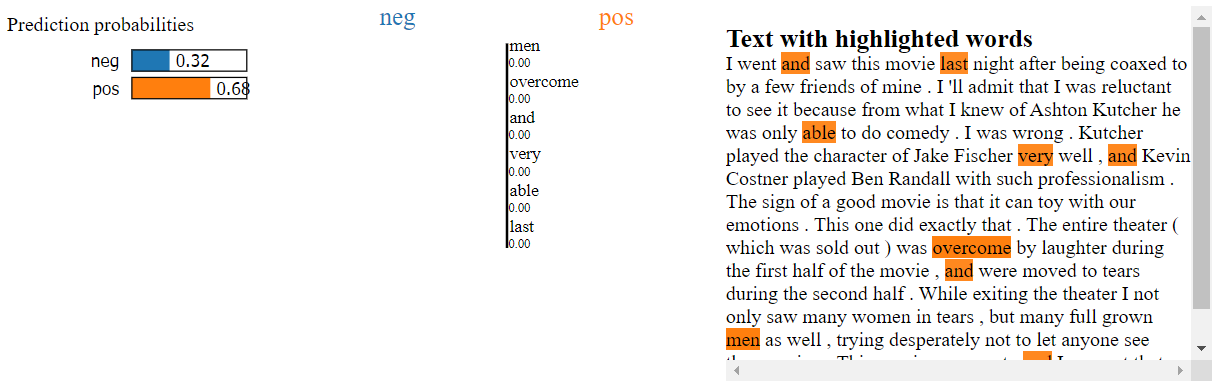
\includegraphics[width=0.95\textwidth]{figures/lime_exp.png}

Подсвеченные слова сильнее всего влияют на результат. Модель отнесла отзыв к положительному классу, основываясь на наличии слов \texttt{and, able, men, last}. Очевидно, что данные слова не влияют на характер отзыва. Таким образом, даже не учитывая значение метрики accuracy, понятно, что модель непригодна для использования, так как совершает предсказания на основе нерелевантных признаков.

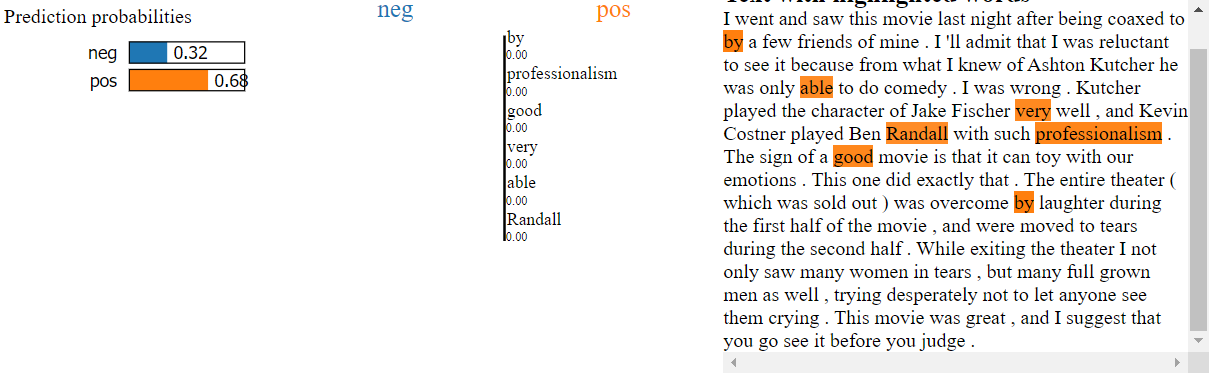
\includegraphics[width=0.95\textwidth]{figures/lime_exp2.png}

Второй пример показывает, что интерпретации несогласованны. А именно, значимые слова отличаются. Такой эффект связан с высокой сложностью рассматриваемой модели.

Вышеперечисленных недостатков мы постараемся избежать в новом подходе.

Для оценки качества интерпретации построим следующие графики:
\begin{itemize}
\item Распределение предсказаний интерпретируемой модели

\item Косинусное расстояние между предсказаниями исходной модели и построенной интерпретируемой модели
\end{itemize}

\section{Анализ ошибки}
Зафиксируем выборку размера 1000. Для каждого объекта сгенерируем похожий объект, заменяя некоторые слова на синонимы. Построим интерпретацию на текущем объекте и предскажем вероятность принадлежности к положительному классу для похожего объекта. Чем меньше полученная вероятность отличается от вероятности, которую предсказывает исходная модель, тем лучше.

Для метода LIME будем строить предсказывать вероятности не на похожем объекте, а на исходном.

\includesvg[width=0.9\textwidth]{../figures/lime_proba_est.svg}

Метод LIME недостаточно точно предсказывает вероятности. График получился шумным, предсказанные вероятность существенно отличаются от истинных значений.

\includesvg[width=0.9\textwidth]{../figures/lime_cosine.svg}

Предсказания, полученные методом LIME, для значительной доли объектов отличается по косинусному расстоянию.

Рассмотрим теперь метод OpenBox.

\includesvg[width=0.9\textwidth]{../figures/openbox_proba_est.svg}

Как видно из графика, есть улучшение по сравнению с методом LIME. Предсказанные вероятности меньше отличаются от исходных.

\includesvg[width=0.9\textwidth]{../figures/openbox_cosine.svg}

График косинусного расстояния также показывает, что интерпретации, полученные методом OpenBox являются согласованными. Есть лишь небольшая доля объектов, на которых наблюдается существенное различие между истинным предсказанием и предсказанием метода.

Вычислим метрики качества.

\begin{tabular}{l|l|l|l}
Метод   &   RMSE  &     MAE &    MAPE\\ \hline
OpenBox & 0.01541 & 0.00849 & 0.01923\\ \hline
LIME    & 0.04085 & 0.01479 & 0.03923\\ \hline
\end{tabular}

Ошибки  метода OpenBox меньше, даже несмотря на то, что измерения для данного метода проводились не на исходных объектах, а на похожих.

\section{Заключение}

В работе был предложен метод выбора интерпретируемой рекуррентной модели глубокого обучения, обладающий свойствами точности и согласованности интерпретаций.

За основу был взят метод OpenBox, предназначенный для интерпретации нейронных сетей с кусочно-линейными функциями активации. 

Было проведено сравнение предложенного метода с методом LIME. Точность и согласованность предложенного метода оказалась выше.

В качестве продолжения данной темы можно рассмотреть нелинейные функции активации (такие как гиперболический тангенс, логистическая сигмоида и т.д.). Если обобщить метод на популярные нелинейные функции активации, то появится способ получать интерпретации для многих известных рекуррентных нейронных сетей.

\bibliographystyle{unsrt}
\bibliography{Gaponov2022InterpretableRNN}

\end{document}
